\documentclass[4paper,12pt]{article}
\usepackage[English]{varioref}
\usepackage{setspace}
\usepackage[margin=2.54cm]{geometry}
\usepackage{pdfpages}
\usepackage[utf8]{inputenc}
\usepackage[english]{babel}
\usepackage{graphicx,subcaption}
\usepackage{graphics}
\usepackage{lscape}
\usepackage{pdflscape}
\usepackage{float}
\usepackage{textcomp}
\usepackage{amsmath}
\usepackage{hyperref}
\usepackage{fancyvrb}
\usepackage{parskip}
\usepackage{changepage}
\usepackage{enumitem}
\usepackage{tcolorbox}
\usepackage[all]{hypcap}
\usepackage{xcolor}
\usepackage{listings}
\definecolor{green}{HTML}{228B22}
\definecolor{orange}{HTML}{FFC107}
\usepackage{color}
\definecolor{dkgreen}{rgb}{0,0.6,0}
\definecolor{gray}{rgb}{0.5,0.5,0.5}
\definecolor{mauve}{rgb}{0.58,0,0.82}
\lstset{escapeinside={<@}{@>}}

\hypersetup{
    colorlinks,
    citecolor=black,
    filecolor=black,
    linkcolor=black,
    urlcolor=black
}


\lstset{frame=tb,
    language=java,
    aboveskip=3mm,
    belowskip=3mm,
    showstringspaces=false,
    columns=flexible,
    basicstyle={\small\ttfamily},
    numbers=none,
    numberstyle=\tiny\color{gray},
    keywordstyle=\color{blue},
    commentstyle=\color{dkgreen},
    stringstyle=\color{mauve},
    breaklines=true,
    breakatwhitespace=true, tabsize=3
}
\title{
	\begin{center}
	\vspace{3cm}
	\includegraphics[width=11cm, height=3cm]{Images/Logo-nou-eps.jpg}
	\end{center}
	\begin{center}
	\line(1,0){340}
	\end{center}		
	DISTRIBUTED COMPUTING\\
	\vspace{2mm}
	\Large Recent advances and new challenges \\
	\line(1,0){340}
	\vspace{2.5cm}
	}

\author{Marc Cervera Rosell - 47980320C \vspace{1cm}}


\date{Academic course 2022 - 2023\vspace{0.5cm} \\Bachelor's degree in computer engineering}
\onehalfspacing

\begin{document}
	\begin{titlepage}
		\maketitle
		\thispagestyle{empty}
	\end{titlepage}
	\cleardoublepage
	\newpage

\tableofcontents
\listoffigures
\thispagestyle{empty}

\newpage
\section*{Question 1}
\addcontentsline{toc}{section}{Question 1}
\subsection*{Identify for each generation the main tech hallmark. Write down the approximate dates for each generation}
\addcontentsline{toc}{subsection}{Identify for each generation the main tech hallmark. Write down the approximate dates for each generation}
\justify{It can be assured that the first computing generation was compressed in the 40's decade, hence the timeline of the first generation is from 1940 to 1950.\\Among a lot of characteristics, the two most highlighted ones are the hardware based on the vacuum tube and the use of magnetic drums and tapes as the main memory.\\ Two examples of computers from this first generation are the ENIAC (Figure ~\ref{fig:ENIAC}) and the IBM 701 (Figure ~\ref{fig:IBM701}).}

\begin{figure}[H]\label{ENIAC}
    \centering
    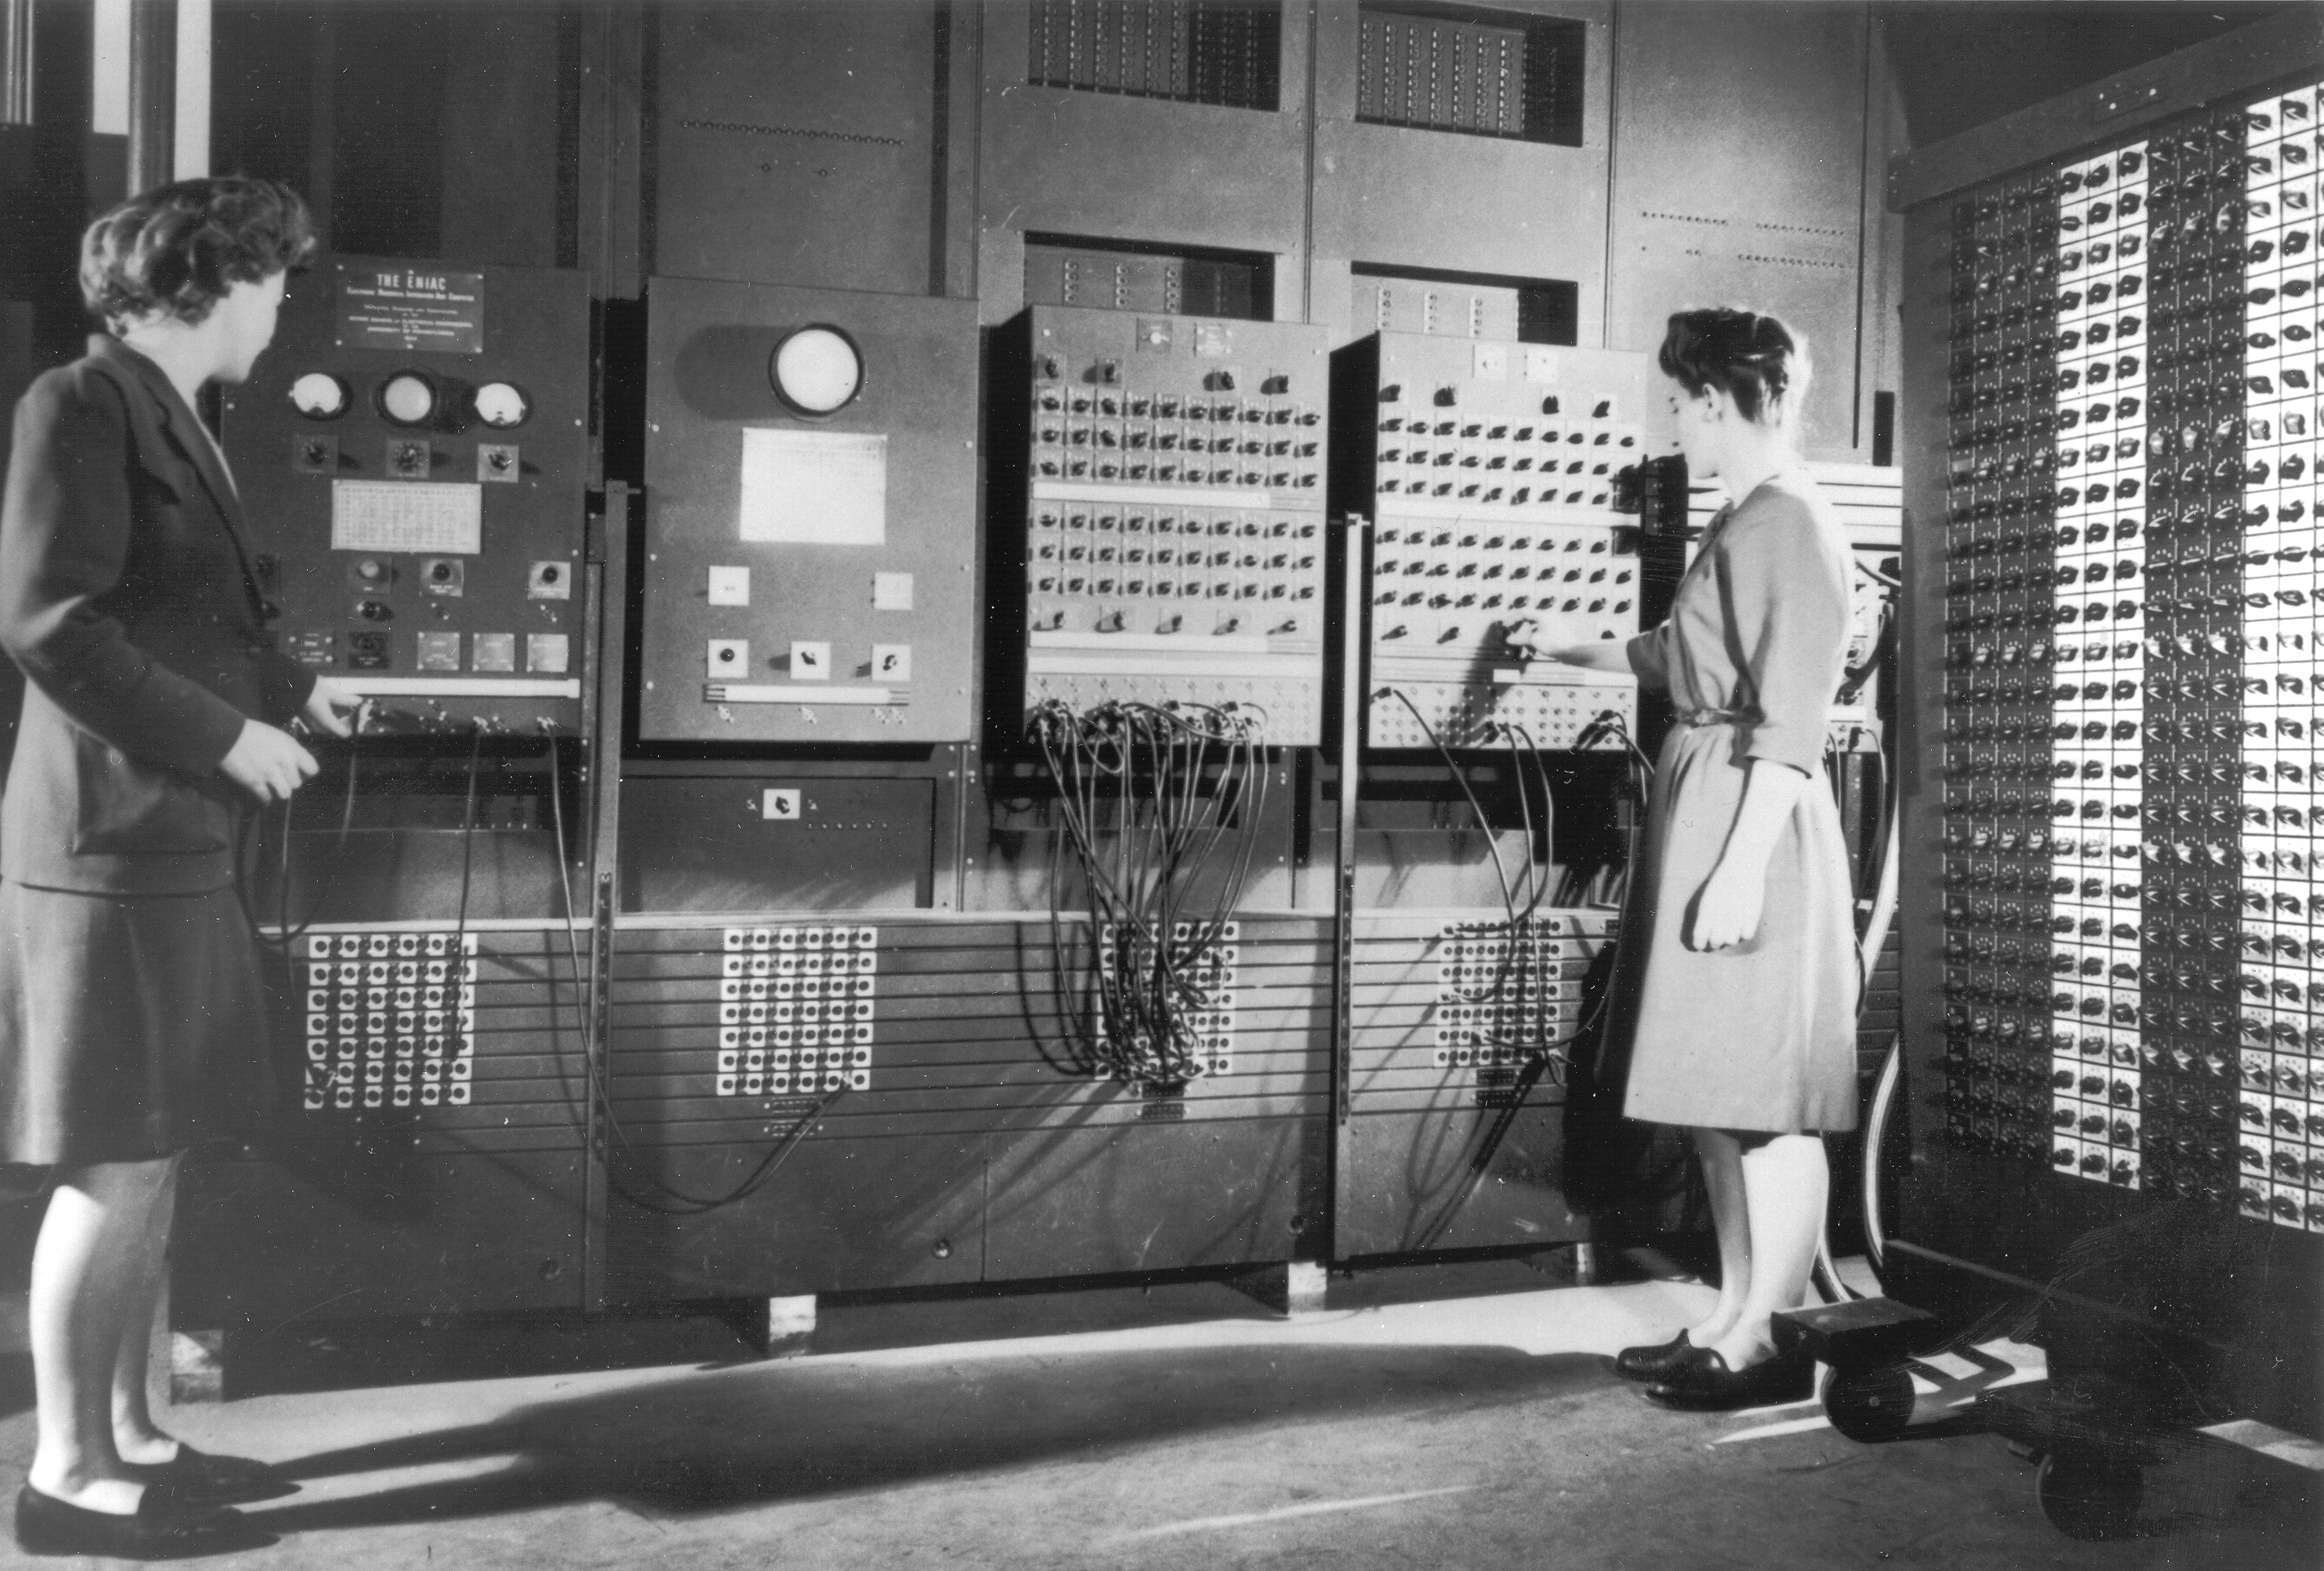
\includegraphics[scale = 0.1]{Images/ENIACArchives.jpg}
    \caption{Computer ENIAC operated by two female operators.}
    \label{fig:ENIAC}
\end{figure}

\begin{figure}[H]
    \centering
    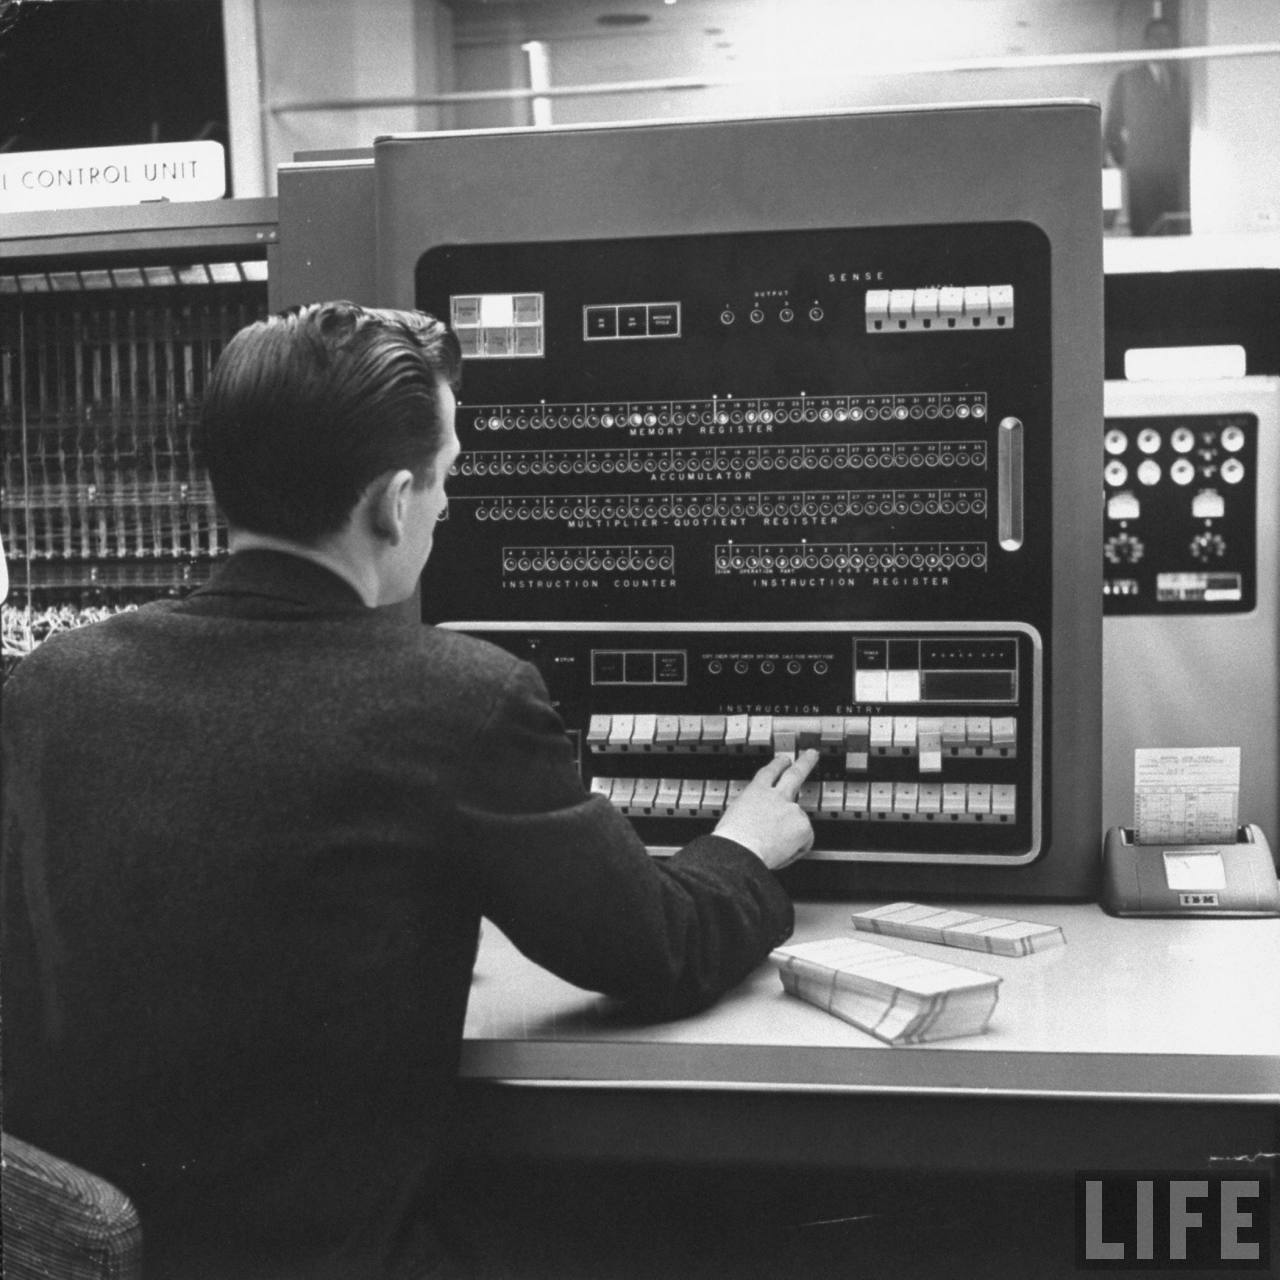
\includegraphics[scale = 0.6]{Images/IBM-701-operator.jpg}
    \caption{IBM 701 operated by a man.}
    \label{fig:IBM701}
\end{figure}

\pagenumbering{arabic}
\newpage
\justify{The second computation generation was compressed between 1950 and 1960.\\The most important change regarding the previous generation is the hardware. In this second generation, the hardware, will not be based on the vacuum tube anymore, It'll be based on transistors. This will behave a reduction of the computer's size. The second most important characteristic is the appearance of the magnetic cores to store information and instructions (magnetic tapes are still used in this generation).\\ Two famous computers of this generation are the IBM 1401 (Figure ~\ref{fig:IBM1401}) and the UNIVAC 1107 (Figure ~\ref{fig:UNIVAC})}

\begin{figure}[H]
    \centering
    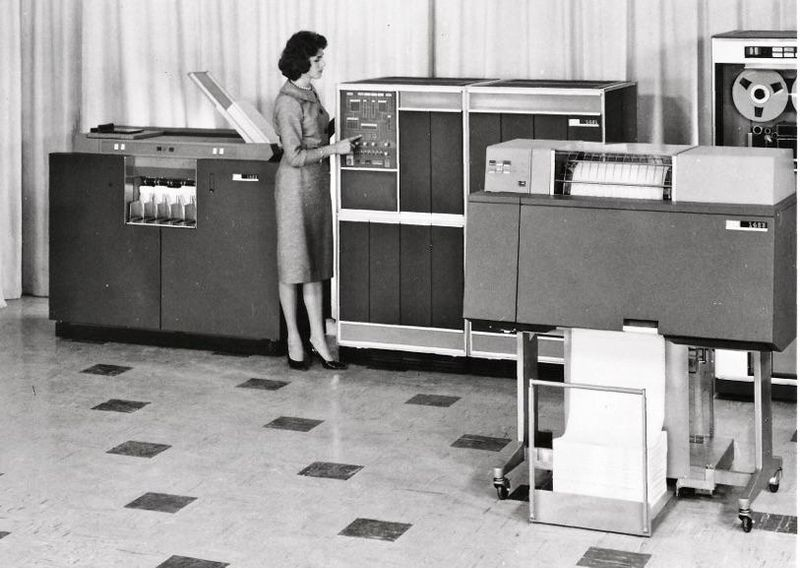
\includegraphics[scale = 0.3]{Images/about-chm-1401_Fig1-PastedGraphic-5.jpg}
    \caption{IBM 1401 operated by a female operator.}
    \label{fig:IBM1401}
\end{figure}

\begin{figure}[H]
    \centering
    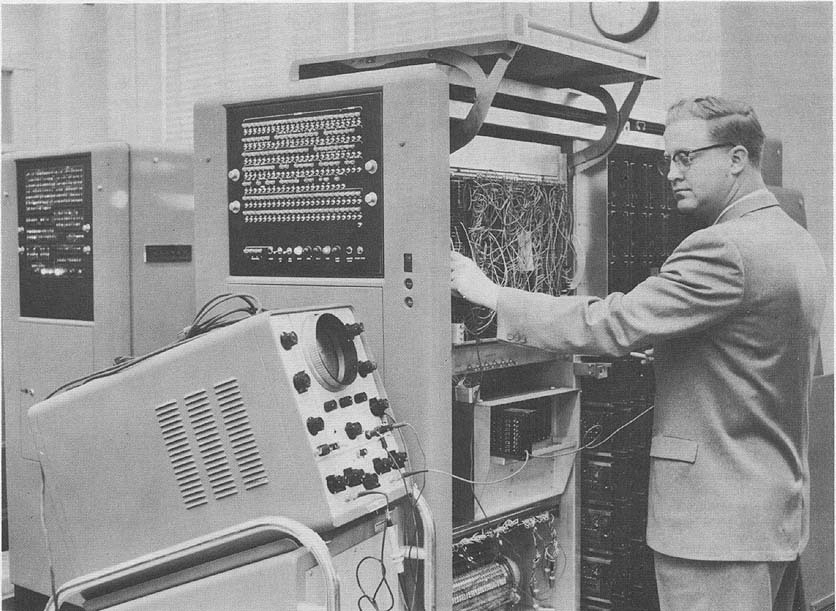
\includegraphics[scale = 0.3]{Images/tumblr_mnh5vyAVUM1r49q4co1_1280.jpg}
    \caption{UNIVAC 1107 operated by a male operator.}
    \label{fig:UNIVAC}
\end{figure}
\newpage
\justify{The third computing generation goes from 1960 to 1970.\\ With this new computer era, they appear the first high level programming languages as are: BASIC, PASCAL, COBOL... and they appear to first "modern" I/O devices such are the keyboard, the monitor, the printer, etc.\\ Of course, there are hardware improvements such are the ICs, but the first high language languages and the modern I/O devices are an inflection point in the computing world.\\ The two most famous computers of this generation are the IBM 360 (Figure ~\ref{fig:IBM360}) and the PDP-11 (Figure ~\ref{fig:PDP11}). }

\begin{figure}[H]
    \centering
    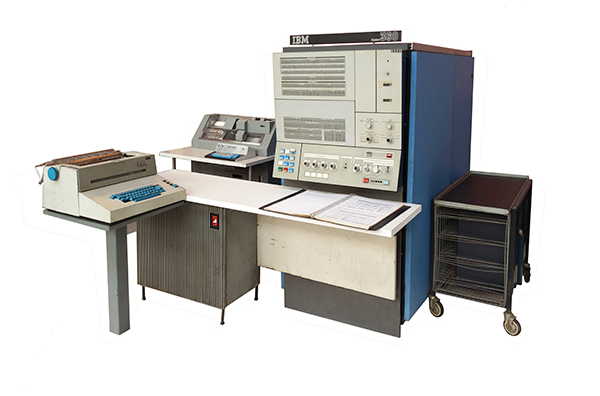
\includegraphics[scale = 0.5]{Images/11470-600x396.jpg}
    \caption{IBM 360}
    \label{fig:IBM360}
\end{figure}

\begin{figure}[H]
    \centering
    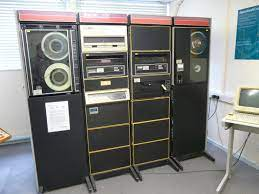
\includegraphics[scale = 0.8]{Images/images.jpg}
    \caption{PDP-11}
    \label{fig:PDP11}
\end{figure}

\newpage
\justify{The fourth generation goes from the 70's to nowadays. This is the actual generation, even thought this generation is starting to die and the fifth generation is starting to "increase his power". One of the main characteristics of this generation is the appearance of the microprocessors and the most important issue of this generation is the appearance possibility of having a group of two or more computer systems linked together, is to say, the appearance of the father of the actual internet, ARPANET.\\ The two most famous computers of this generation are the IBM PC (Figure ~\ref{fig:IBMPC}) and the APPLE II (Figure ~\ref{fig:appleII}).}

\begin{figure}[H]
    \centering
    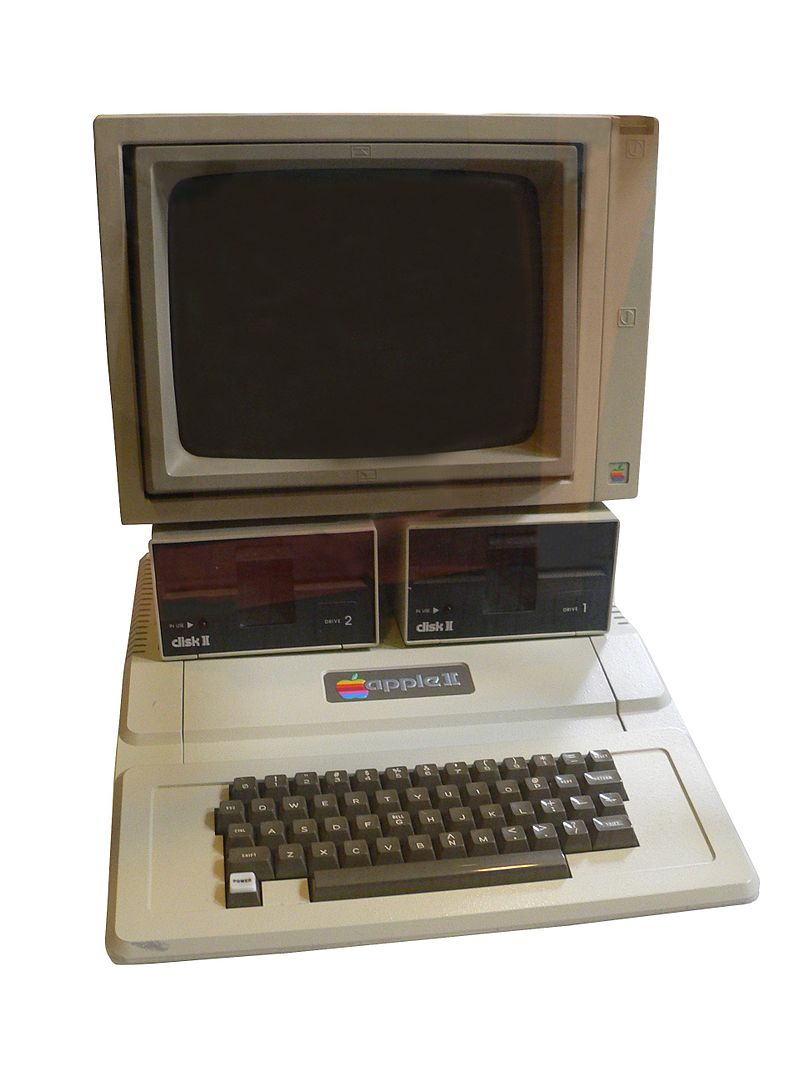
\includegraphics[scale = 0.2]{Images/800px-Apple-II.jpg}
    \caption{Apple II}
    \label{fig:appleII}
\end{figure}

\begin{figure}[H]
    \centering
    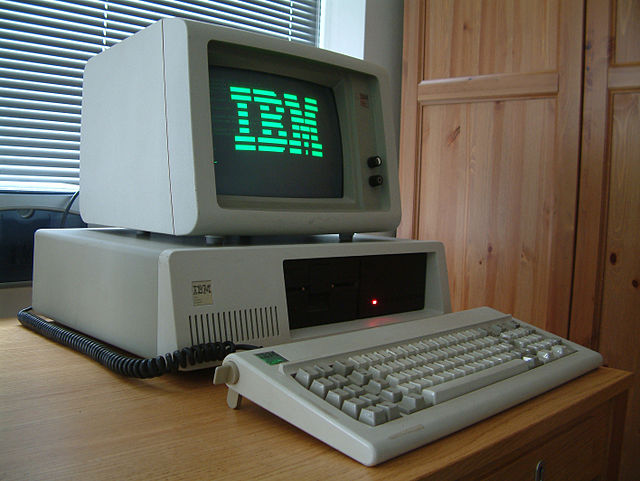
\includegraphics[scale = 0.4]{Images/Ibm_px_xt_color.jpg}
    \caption{IBM PC}
    \label{fig:IBMPC}
\end{figure}

\justify{The fifth and the last generation (for the moment) is the future generation, but it's starting to be the current generation. The main characteristics of this era are the hardware based on AI using the ultra large-scale integration and the parallel processing method. And the second main characteristic is the capacity of understanding the natural/human language. Examples of computers from this generation are the desktops, laptops, smartphones, tablets, etc.}

\section*{Question 2}
\addcontentsline{toc}{section}{Question 2}
\subsection*{In your opinion, which are the hallmarks during the 1990's?}
\addcontentsline{toc}{subsection}{In your opinion, which are the hallmarks during the 1990's?}
\justify{The most important hallmark in the 90's was the world wide web. In fact, on December 20th, 1990, the first web-page was published, and It was quite rudimentary, specially compared to what we've today.\\ The second most important hallmark in the 90's was the appearance of the Linux operating system. Linux, is maybe the most known open-source operating system. According to Stack Overflow's survey, Linux is the most popular development platform with the $48.3\%$ of the votes. The 90's decade, had other very important hallmarks as is the e-commerce, the invention of the USB flash drives, the invention of Java, etc. }
\subsection*{In your opinion, which are the hallmarks at the beginning of this century?}
\addcontentsline{toc}{subsection}{In your opinion, which are the hallmarks at the beginning of this century?}
\justify{One of the most important tech improvements at the beginning of the century was the appearance of a new short-range wireless technology called Bluetooth. This technology is still used nowadays (it's one of the most important short-range wireless technology). Bluetooth 1.0 was launched in 1999, however it wasn't until 2000 when product began to incorporate it. The Ericsson T36 was the first mobile phone with this technology.\\ Another important hallmark was a new operating system called Android. This operating system was launched in 2008 and was to become one of the most important operating systems for mobile phones.}
\subsection*{In your opinion, which are the hallmarks nowadays?}
\addcontentsline{toc}{subsection}{In your opinion, which are the hallmarks nowadays?}
\justify{Even thought the concept of "Quantum computing" exists since the 80's, It hasn't been very popular until now. Personally, I think that the "Quantum computing" can be considered a hallmark of our era because in 2011 was sold the first quantum computer. The fact of selling something, means that is able to do some service for the society.\\ Another hallmark of our era, is the capacity to apply the AI in different areas such are the healthcare, banking, education, agriculture, gaming, space exploration, military, etc. }

\section*{Question 3}
\addcontentsline{toc}{section}{Question 3}
\subsection*{Which are the main differences between hallmarks (1990-2020) and the tech hallmarks on the previous generations (First to Forth)?}
\addcontentsline{toc}{subsection}{Which are the main differences between hallmarks (1990-2020) and the tech hallmarks on the previous generations (First to Forth)?}
\justify{The most evident difference is the size of the machines. The more you go back in the time, the more the size of the computers increases. The first computers in history needed an entire room and the actual computers only need no more than a table.\\ The second main difference is the hardware of the machines. At the beginning computers were using vacuum tubes and now are starting to use AI.\\ One of the most important hallmarks is the transition from analogue technology to digital technology.\\ The I/O devices are also a very important hallmark, because the computing has passed from use magnetic tapes to use USB flash devices, hard disks, SSD, memory cards...\\ There are more differences among the generation but these are the most important ones.}

\section*{Question 4}
\addcontentsline{toc}{section}{Question 4}
\subsection*{When we increase the number of transistors per unit space so disproportionately, what two main challenges must be faced?}
\addcontentsline{toc}{subsection}{When we increase the number of transistors per unit space so disproportionately, what two main challenges must be faced?}
\justify{As it is known the Moore's law is the law that affirms that every two years, the number of transistors in a dense integrated circuit will be doubled.}
\justify{The first challenge that has to be faced are the physical limits of the current technology. The more the density of the transistors increases the more heat increases. Hence, is not possible to extract the heat fast enough, and this creates a risk of over-heating and damaging the microprocessor. In addition, normally the transistors become smaller to increase the amount of these in the chips, without changing the size of the chip, which has a physical limit imposed by the size of the atoms.\\ The second challenge is the reduction of the prices at the same time that the performance increases. This means that if somebody buys a computer today, the next year the same computer will cost half and in two years that same computer will be outdated.}

\section*{Question 5}
\addcontentsline{toc}{section}{Question 5}
\subsection*{Do you think that the curve is representing the natural growing of transistors in integrated circuits, or that the manufactures are doing something special to maintain this behavior?}
\addcontentsline{toc}{subsection}{Do you think that the curve is representing the natural growing of transistors in integrated circuits, or that the manufactures are doing something special to maintain this behavior?}
\justify{In my opinion, the curve is not representing the natural growing of transistors in ICs for two reasons:}

\begin{enumerate}
    \item There exist physical limitations imposed by the atom's size. So, or manufactures stop adding transistors in the ICs or if they want to continue increasing the number of transistors, will arrive a moment that they'll have to increase the ICs size.
    \item The manufactures are searching software solutions instead of hardware solutions. As it is to say, manufactures are searching software solutions to avoid the physical limits.
\end{enumerate}

\section*{Question 6}
\addcontentsline{toc}{section}{Question 6}
\subsection*{When would you date the appearance of the first distributed application?}
\addcontentsline{toc}{subsection}{When would you date the appearance of the first distributed application?}
\justify{A distributed application is defined as a collection of autonomous components linked by a network. According to this definition, I would date the first distributed application in 1844. In that year Samuel Morse invented the telegraph. Personally, I think that It's a great example of a distributed application, because It has all the necessary to be one. Were the telegraphs a collection of autonomous components? Yes, every city had at least one telegraph. Were the telegraphs linked by a network? Yes, they were linked by the electrical network. Were the telegraphs had a software? Yes, the Morse code was the used software.}

\section*{Question 7}
\addcontentsline{toc}{section}{Question 7}
\subsection*{During the nineties until now were created different architectures (different
to the usual Client/Server) that takes profit of the joint computing power and sharing of distributed resources. Can you mention some of these architectures?}
\addcontentsline{toc}{subsection}{During the nineties until now were created different architectures (different to the usual Client/Server) that takes profit of the joint computing power and sharing of distributed resources. Can you mention some of these architectures?}
\begin{itemize}
    \item Client-Server architecture
    \item Broken pattern architecture
    \item Service-oriented architecture
    \item n-tier architecture
    \item Peer-to-peer
\end{itemize}

\section*{Question 8}
\addcontentsline{toc}{section}{Question 8}
\subsection*{At the beginning of the XXI century, some authors said that the big challenges will be the Artificial Intelligence, Robotics, Expert Systems, communication infrastructures, molecular computers, etc. In your opinion, What are the current most important challenges for manufacturers and governments in the field of computing?}
\addcontentsline{toc}{subsection}{At the beginning of the XXI century, some authors said that the big challenges will be the Artificial Intelligence, Robotics, Expert Systems, communication infrastructures, molecular computers, etc. In your opinion, What are the current most important challenges for manufacturers and governments in the field of computing?}
\justify{As we are in a capitalist system, all business bosses, search to win the major amount of money without having to pay a lot for the workers. So, the manufactures have the challenge to replace human workers for AI based systems/robots that they do the same work by free and better. But with the technology that exists nowadays is not possible to replace all the human workers for AI based systems/robots, even though there are work places that have been conquered by the robots.\\ Another challenge for manufactures is digitize the maximum number of processes that require (for now) a human actuation.\\ Switching to the government area, the most important challenge in computing is to create systems to protect the country. Is it to say, every country has an intelligence center (Spain's case is the CNI), so the challenge is to create systems that allow the agents of the intelligence center protect the country with making the less possible stir. Keeping in the government area, the military part is an important one, because every army of every country around the world has a scientific team working in computing projects (usually of espionage and counterespionage), in healthcare projects, in weapon projects, etc.}

\end{document}
